%%% Local Variables:
%%% mode: latex
%%% TeX-master: "<none>"
%%% End:

\label{sec:joining}

After connecting with a splitter, incoming peers request (using a
reliable communication) to the splitter the current list of peers in
the team. To minimize the joining time, the peer sends a
$[\mathtt{hello}]$ \emph{message} to each other peer of the team, in
parallel with the reception of the list. When a peer of the team
receives a $[\mathtt{hello}]$, it adds the sender of the message to a
table of peers called $\mathtt{forward}[]$ \note{(see
  \href{https://github.com/P2PSP/simulator/blob/f0c73be1817e7d3b816cc61cd2c8e59b17f9a0e6/src/core/peer_dbs.py\#L491}{$\text{forward[]}$
    in \texttt{peer.py}})}. If a peer $P_i$ has an entry
$\mathtt{forward}[P_j]=P_k$, then each chunk received by $P_i$ and
originated at $P_j$ will be forwarded to $P_k$. When an incoming peer
$P_i$ has received the list of peers, its forwarding table has been
initialized to $\mathtt{forward}[P_i]=\{\text{team}\}$. Notice that,
as long as the forwarding table contains this information, all chunks
received from the splitter will be forwarded to the rest of the team.

%), initializes
%the table $\mathrm{debt}[]$ (which stores the chunk debts between
%neighbor peers), and (3) sets the variable $\mathrm{neighbor}$ with an
%index to $\mathrm{forward}[]$ (see
%Sec.~\ref{sec:chunk_DBS_processing}).

The splitter, in an infinite loop: (1) listens to the incoming peers,
(2) sends to them the list of peers in the team, and (3) adds the
incoming peer to the list. Notice that only those peers that are in
the list of peers of the splitter are considered to be in the team
served by such splitter.

\begin{comment}
\begin{figure*}
  %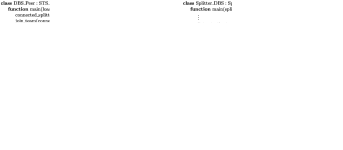
\includegraphics[width=\textwidth]{joining}
  \fig{1000}{10cm}{joining} \caption{Code related to team
    joining.\label{fig:joining}}
\end{figure*}

The new pseudo-code related to joining a team is describen in the
Fig.~\ref{fig:joining}.
\end{comment}

\begin{notex}
  See \href{https://github.com/P2PSP/simulator/blob/f0c73be1817e7d3b816cc61cd2c8e59b17f9a0e6/src/core/splitter_dbs.py#L296}{$\text{destination\_of\_chunk}[]$ in \texttt{peer\_dbs.py}}.
\end{notex}
